\section{Method}
The workflow consisted of three main routines: feature extraction, vegetation classification, and linear object segmentation (figure \ref{fig:workflow}). Each of these is explained in more detail below.

\begin{figure}
	\centering
	\begin{tikzpicture}[node distance=0.70cm, scale=0.7, every node/.style={transform shape}]

	\node (pro0) [process, fill=darkorange!20] {Point-based feature extraction};
	\node (pro1) [process, right=of pro0, fill=darkorange!20] {Neighborhood-based geometry feature extraction};
	\node (pro2) [process, right=of pro1, fill=darkorange!20] {Neighborhood-based eigenvalue feature extraction};

	\node (param) [title, above=0.4cm of pro1] {Feature extraction};

	\begin{scope}[on background layer]
	\node (fit1) [fit=(pro0)(pro1)(pro2)(param), inner sep=4pt, transform shape=false, draw=black!80, fill=darkorange, fill opacity=0.5] {};
	\end{scope}

	\node (in1) [io, left=of fit1] {Unclassified point cloud};
	\node (out1) [io, below right=0.9cm and 11.7cm=of fit1] {Point cloud with features};

	\node (class) [title, below=1.2cm of pro1] {Vegetation classification};

	\node (pro5) [process, below=0.2cm of class, fill=lightblue!20] {Supervised classification (random forest)};
	\node (pro4) [process, right=of pro5, fill=lightblue!20] {Data trimming};
	\node (in2) [io, below=of pro5] {Manually classified point cloud};
	\node (pro6) [process, left=of pro5, fill=lightblue!20] {Accuracy assessment (cross validation)};

	\begin{scope}[on background layer]
	\node (fit2) [fit=(class)(pro4)(pro5)(pro6), inner sep=4pt, transform shape=false, draw=black!80, fill=lightblue, fill opacity=0.5] {};
	\end{scope}

	\node (out2) [io, below left=4.9cm and 3.7=of fit2] {Classified point cloud};

	\node (lin) [title, below=of in2] {Linear object segmentation};
	\node (pro11) [process, below=0.2cm of lin, fill=turquoise!20] {Clustering (using DBSCAN)};
	\node (pro10) [process, left=of pro11, fill=turquoise!20] {Preprocessing (2D conversion and downsampling)};
	\node (pro12) [process, right=of pro11, fill=turquoise!20] {Region growing (based on rectangularity)};
	\node (pro13) [process, below=of pro10, fill=turquoise!20] {Object merging};
	\node (pro14) [process, right=of pro13, fill=turquoise!20] {Elongatedness assessment};
	\node (pro15) [process, right=of pro14, fill=turquoise!20] {Accuracy assessment};


	\begin{scope}[on background layer]
	\node (fit3) [fit=(lin)(pro10)(pro11)(pro12)(pro13)(pro14)(pro15), inner sep=4pt, transform shape=false, draw=black!80, fill=turquoise, fill opacity=0.5] {};
	\end{scope}

	\node (in3) [io, below=of pro15] {Manually segmented vegetation objects};

	\node (out3) [io, right=of fit3] {Linear vegetation objects};
%	\node (out3) [io, right=3.2cm of pro14] {Linear vegetation objects};

	\draw [arrow] (in1) -- (fit1);
	\draw [arrow] (fit1) -| (out1);
	\draw [arrow] (out1) |- (fit2);
	\draw [arrow] (in2) -- (fit2);

	\draw [arrow] (pro0) -- (pro1);
	\draw [arrow] (pro1) -- (pro2);

	\draw [arrow] (pro4) -- (pro5);
	\draw [arrow] (pro5) -- (pro6);
	\draw [arrow] (pro6) -- (pro5);

	\draw [arrow] (fit2) -| (out2);
	\draw [arrow] (out2) |- (fit3);

	\draw [arrow] (pro10) -- (pro11);
	\draw [arrow] (pro11) -- (pro12);
	\draw [arrow] (pro12.south) -| +(0,-0.3) -| (pro13.north);
	\draw [arrow] (pro13) -- (pro14);
	\draw [arrow] (pro14) -- (pro15);

	\draw [arrow] (in3) -- (in3 |- fit3.south);

	\draw [arrow] (fit3) -- (out3);
%	\draw [arrow] (out3 -| fit3.east) -- (out3);

	\end{tikzpicture}
	\caption{Workflow for feature extraction (orange), vegetation classification (blue), and linear objects segmentation (green). Computational steps are represented as rectangles and datasets as parallelograms.}
	\label{fig:workflow}
\end{figure}

\subsection{Feature extraction}

The relevance of the various input features has been extensively studied to separate urban from vegetation objects \citep{chehata2009airborne, guo2011relevance, mallet2011relevance}, but concise information for vegetation classification is scarce. After reviewing relevant literature, we selected fourteen features (table \ref{tbl:features}) which were later used for classification. These features are grouped in point-based and neighborhood-based features and reflect information from echo and local neighborhoods (geometric and eigenvalue based), respectively. The qualities of these features are considered to be efficient for discriminating vegetation objects from point clouds \citep{chehata2009airborne}.

\subsubsection{Point-based features}
The point-based features represent information from each single point (table \ref{tbl:features}). The point cloud \(\mathcal{P}\) is a set of points \(\{p_{1}, p_{2}, \dots, p_{n}\}\) \(\in \mathbb{R}^3\), where each point \(p_{i}\) has x, y and z coordinates. In addition, an intensity value (\(I\)), a return number (\(R\)), and a number of returns (\(R_{t}\)) of the returned signal are stored. We used \(R_{t}\) as well as the normalized return number \(R_{n}\) as echo-based features (table \ref{tbl:features}). Since the available LiDAR data were lacking the information required to do a radiometric correction of the intensity data we omitted this feature for the classification \citep{kashani2015review}.

\subsubsection{Neighborhood-based features}
In addition to point-based features, we computed features based on the local neighborhoods of the points. We defined a neighborhood set \(\mathcal{N}_{i}\) of points \(\{q_{1}, q_{2}, \dots, q_{k}\}\) for each point \(p_{i}\), where \(q_{1} = p_{i}\), by using the k-nearest neighbors method with \(k = 10\) points. In this way a k of 10 results in a neighborhood of ten points, one of which is the concerned point itself. Based on these neighborhoods we then computed four geometric features: height difference, height standard deviation, local radius and local point density (table \ref{tbl:features}).

In addition to these geometric features we further calculated eight eigenvalue-based features (table \ref{tbl:features}), which are used to describe the distribution of points of a neighborhood in space \citep{hoppe1992surface, chehata2009airborne}. We used the local structure tensor to estimate the surface normal and to define surface variation \citep{pauly2002efficient}. The structure tensor describes the dominant directions of the neighborhood of a point by determining the covariance matrix of the x, y and z coordinates of the set of neighborhood points and computing the eigenvalues (\(\lambda_{1}, \lambda_{2}, \lambda_{3}\), where \(\lambda_{1} > \lambda_{2} > \lambda_{3}\)) of this matrix and ranking them based on the eigenvalue values. Hence, the magnitude of the eigenvalues of this covariance matrix describe the spread of points in the direction of the eigenvector. The eigenvector belonging to the third eigenvalue is equal to the normal vector (\(\vec{N} = (N_{x}, N_{y}, N_{z})\)) \citep{pauly2002efficient}. The points are linearly distributed if the eigenvalue of the first principle direction is significantly larger than the other two (\(\lambda_{1} \gg \lambda_{2} \approx \lambda_{3}\)), planarly distributed if the eigenvalues of the first two principle directions are about equal and significantly larger than the third (\(\lambda_{1} \approx \lambda_{2} \gg \lambda_{3}\)), and the points are scattered in all directions if all eigenvalues are about equal (\(\lambda_{1} \approx \lambda_{2} \approx \lambda_{3}\)). These properties (linearity, planarity and scatter), as well as some additional features (omnivariance, eigenentropy, sum of eigenvalues and curvature), are quantified using formulas (table \ref{tbl:features}).

\begin{table}[t]
	\caption{The features used for classification, split into two main groups: point-based and neighborhood-based. The point-based features are based on echo information and the neighborhood-based features are based on the local geometry and eigenvalue characteristics.}
	\label{tbl:features}
	\footnotesize
	\begin{tabular}{l l l l l}
		\toprule
		\textbf{Feature group} & \textbf{Feature} & \textbf{Symbol} & \textbf{Formula} & \textbf{Reference} \\
		\midrule
		\textbf{Point} \\ \\
		- Echo & Number of returns & \(R_{t}\) & \\ \\
		& Normalized return number & \(R_{n}\) & \(R/R_{t}\) & \citet{guo2011relevance} \\ \\
		\textbf{Neighborhood} \\ \\
		- Geometric & Height difference & \(\Delta_{z}\) & \(\max_{j:\mathcal{N}_{i}}(q_{z_{j}}) - \min_{j:\mathcal{N}_{i}}(q_{z_{j}})\) & \cite{weinmann2015semantic} \\ \\
		& Height standard deviation & \(\sigma_{z}\) & \(\sqrt{\frac{1}{k} \sum_{j=1}^k (q_{z_{j}} - \overline{q_{z}})^2}\) & \cite{weinmann2015semantic} \\ \\
		& Local radius & \(r_{l}\) & \(\max_{j: \mathcal{N}_{i}}(|p_{i} - q_{j}|)\) & \cite{weinmann2015semantic} \\ \\
		& Local point density & \(D\) & \(k/(\frac{4}{3} \pi r_{l}^3)\) & \cite{weinmann2015semantic} \\ \\
		- Eigenvalue & Normal vector Z & \(N_{z}\) & & \citet{pauly2002efficient} \\ \\
		& Linearity & \(L_{\lambda}\) & \(\frac{\lambda_{1} - \lambda_{2}}{\lambda_{1}}\) & \citet{west2004context} \\ \\
		& Planarity & \(P_{\lambda}\) & \(\frac{\lambda_{2} - \lambda_{3}}{\lambda_{1}}\) & \citet{west2004context} \\ \\
		& Scatter & \(S_{\lambda}\) & \(\frac{\lambda_{3}}{\lambda_{1}}\) & \citet{west2004context} \\ \\
		& Omnivariance & \(O_{\lambda}\) & \(\sqrt[3]{\lambda_{1} \lambda_{2} \lambda_{3}}\) & \citet{west2004context} \\ \\
		& Eigenentropy & \(E_{\lambda}\) & \(-\lambda_{1}\ln(\lambda_{1}) -\lambda_{2}\ln(\lambda_{2}) -\lambda_{3}\ln(\lambda_{3})\) & \citet{west2004context} \\ \\
		& Sum of eigenvalues & \(\sum_{\lambda}\) & \(\lambda_{1} + \lambda_{2} + \lambda_{3}\) & \cite{mallet2011relevance} \\ \\
		& Curvature & \(C_{\lambda}\) & \(\frac{\lambda_{3}}{\lambda_{1} + \lambda_{2} + \lambda_{3}}\) & \citet{pauly2002efficient} \\ \\
		\bottomrule
	\end{tabular}
\end{table}

\subsection{Vegetation classification}
The fourteen features (two echo, four geometric, and eight eigenvalue features) served as input for the vegetation classification. For this we first trimmed irrelevant points, then used a supervised classification to classify the remaining points, and finally assessed the accuracy.

\subsubsection{Data trimming}
To facilitate efficient processing, points that clearly did not belong to tall vegetation were removed from the dataset. This was done to remove non-vegetation and low-stature vegetation (e.g. grasses, herbs, agricultural fields) and to allow identification of linear vegetation elements with a certain height (i.e. composed of shrubs and trees). The points to be removed were characterized by a locally planar neighborhood and selected on the basis of the scatter feature (table \ref{tbl:features}). Points with a very low scatter value (\(S_{\lambda} < 0.03\)) were removed, as this threshold was conservative and allowed to reduce thee data size, while still preserving all points characterizing tall vegetation.

\subsubsection{Supervised classification}
For the vegetation classification, we used a random forest classifier because it provides a good trade-off between classification accuracy and computational efficiency \citep{breiman2001random, weinmann2015semantic}. The random forest algorithm creates a collection of decision trees, where each tree is based on a random subset of the training data \citep{ho1998random}. Random forest parameters such as the maximum number of features, minimal samples per leaf, minimal samples per split and the ratio between minority and majority samples were optimized using a grid search. During the grid search a range of applicable values were chosen for each parameter and all combinations were tested and evaluated for performance using cross validation. To save time first a course grid (meaning the values of the parameters were in a larger range and more distance in between) was created to identify the region of best performance and subsequently a finer grid was made to find the best performing parameter set in that region \citep{hsu2003practical}.

As the trimmed point cloud was imbalanced (i.e. it included a lot more \textit{vegetation} than \textit{other} points) and imbalanced training data can lead to undesirable classification results \citep{he2009learning}, we used a balanced random forest algorithm. In this algorithm the subsets are created by taking a bootstrap sample from the minority class and a random sample from the majority class with a size based on the size of the minority class sample \citep{chen2004using}. By employing enough trees all majority class data are eventually used, while still maintaining a balance between the two classes. The decision trees were created using a Classification and Regression Tree (CART) algorithm \citep{breiman1984classification}. 

\subsubsection{Accuracy assessment}
For the accuracy assessment of the vegetation classification, a manual annotation of the trimmed point cloud into \textit{vegetation} (e.g. trees and shrubs) and \textit{other} (e.g. buildings, ditches, railroad infrastructure) classes was done using an interpretation of the point cloud and high resolution aerial photos. This resulted in a ground truth dataset of 101226 points of \textit{vegetation} and 57752 points of \textit{other}. To allow for a good assessment of the performance, while considering the imbalance in the dataset, we used the receiver operating characteristic (ROC) curve \citep{bradley1997use}, the Matthew’s correlation coefficient (MCC) \citep{matthews1975comparison} and the geometric mean \citep{kubat1998machine} as accuracy metrics. These metrics evaluate the performance of a classifier well, even when dealing with an imbalanced dataset \citep{kohavi1995study, sun2009classification, lopez2013insight}. To create a ROC curve, the true positive (TP) rate is plotted against the false positive (FP) rate at various decision thresholds. The area under a ROC curve (AUROCC) is a measure for the performance of the classifier \citep{bradley1997use}. The MCC analyzes the correlation between the observed and the predicted data and is defined as:
\begin{equation}
	\label{eq:MCC}
	{\text{MCC}}={\frac{TP\times TN-FP\times FN}{{\sqrt{(TP+FP)(TP+FN)(TN+FP)(TN+FN)}}}}
\end{equation}
where TN are the true negatives and FN the false negatives. The geometric mean is defined as:
\begin{equation}
	\label{eq:geom}
	{\text{Geometric mean}}={\sqrt{\frac{TP}{TP+FP} \times \frac{TN}{TN+FN}}}
\end{equation}

The MCC, AUROCC and the geometric mean were obtained using a 10-fold cross validation. This is done by splitting the data into 10 randomly mutually exclusive subsets and using a subset as testing data and a classifier trained on the remaining data \citep{kohavi1995study}.

\subsection{Linear object segmentation}
For the third part of the workflow (linear object segmentation), we applied a preprocessing step, clustered the points, applied a region growing algorithm, merged nearby and aligned objects, evaluated their elongatedness, and finally assessed the accuracy (figure \ref{fig:workflow}).

\subsubsection{Preprocessing}
Since we defined linearity as a purely two dimensional property, the point cloud was converted to 2D by removing the z-coordinate of the vegetation points. In addition, the data were spatially downsampled to 1 meter distance between vegetation points using Poisson sampling. Without losing too much precision (figure \ref{fig:downsampling}), this substantially decreased computation time.

\begin{figure}
	\centering
	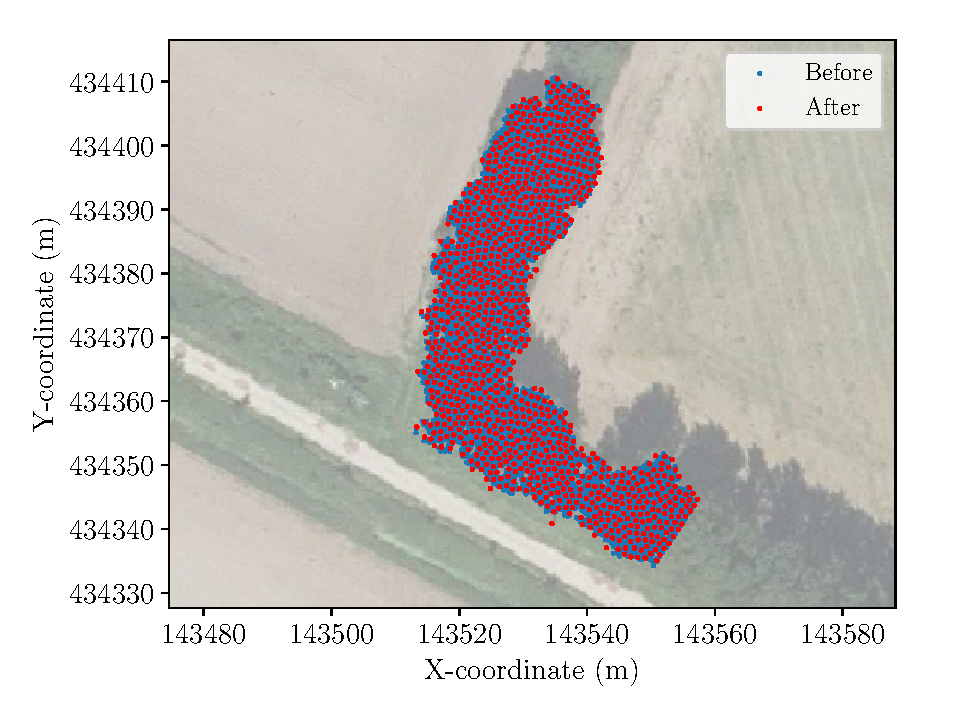
\includegraphics[scale=0.80]{./img/downsampling.pdf}
	\caption{The vegetation points of a piece of tree line within the research area before (blue) and after (red) downsampling the point cloud, plotted on top of the high resolution orthophoto, in RD coordinates.}
	\label{fig:downsampling}
\end{figure}

\subsubsection{Clustering}
After reducing the amount of points, we clustered the remaining points together using a DBSCAN clustering algorithm \citep{ester1996density}. This algorithm is able to quickly cluster points together based on density and removes outlying points in the process. This decreased the processing time needed in the subsequent region growing step, since the amount of possible neighboring points is reduced.

\subsubsection{Region growing}
Region growing is an accepted way of decomposing point clouds \citep{rabbani2006segmentation, vosselman2013point} into homogeneous objects. Normally, regions are grown based on similarity of the attributes of the points. Here, regions were grown based on a rectangularity constraint. The rectangularity of an object is described as the ratio between the area of an object and the area of its minimum oriented bounding box (MOBB) \citep{rosin1999measuring}. The MOBB (figure \ref{fig:hulls}b) is computed using rotating calipers \citep{toussaint1983solving}. Here first a convex hull (figure \ref{fig:hulls}a) is constructed using the QuickHull algorithm \citep{preparata1985computational} and then the MOBB can be found by rotating the system by the angles the edges of the convex hull make with the x-axis and checking the bounding rectangles of each rotation, as the minimum oriented bounding box has a side collinear with one of the edges of the convex hull \citep{freeman1975determining}. The area of the object can be calculated by computing the concave hull of the set of points belonging to the object (figure \ref{fig:hulls}c). This hull is found by computing an alpha shape of the set of points \citep{edelsbrunner1983shape}. This shape is created by computing a Delaunay triangulation of the points \citep{delaunay1934sphere} and removing the triangles with a circumradius higher than \(1/\alpha\), where \(\alpha\) is a parameter which consequently influences the amount of triangles removed from the triangulation and thus the shape and area of the alpha shape. Higher alphas lead to more complex shapes, while lower ones to more smooth shapes.

% For this we use a concave hull algorithm using a \(k\)-nearest neighbors approach \citep{moreira2007concave}. This algorithm starts with finding a point with a minimum or maximum of one of the coordinates. Subsequently it goes around the points by repeatably finding the neighbor which makes an edge that makes the largest counterclockwise angle with the previous edge. This process is continued until the current point is the starting point. Finally a check is done to ensure all the points fall within the hull. If this is not the case the \(k\) is increased by 1 and the algorithm repeated until an acceptable concave hull has been found.

For each cluster, points with the minimum x-coordinate and its ten closest neighbors were used as the starting region. Subsequently for each point the eight nearest neighbors are considered for growth (figure \ref{fig:regiongrowing}). Points were added as long as the region's rectangularity did not drop below a set threshold. An analysis of this threshold value on a subset of the data showed the best performance of the algorithm when this value was between 0.5 and 0.6, with marginal differences in performance in between these values, so we set it at 0.55. After a region is grown, the growing procedure was repeated for the next region until the entire cluster is segmented into rectangular regions.

%\begin{figure}
%	\centering
%	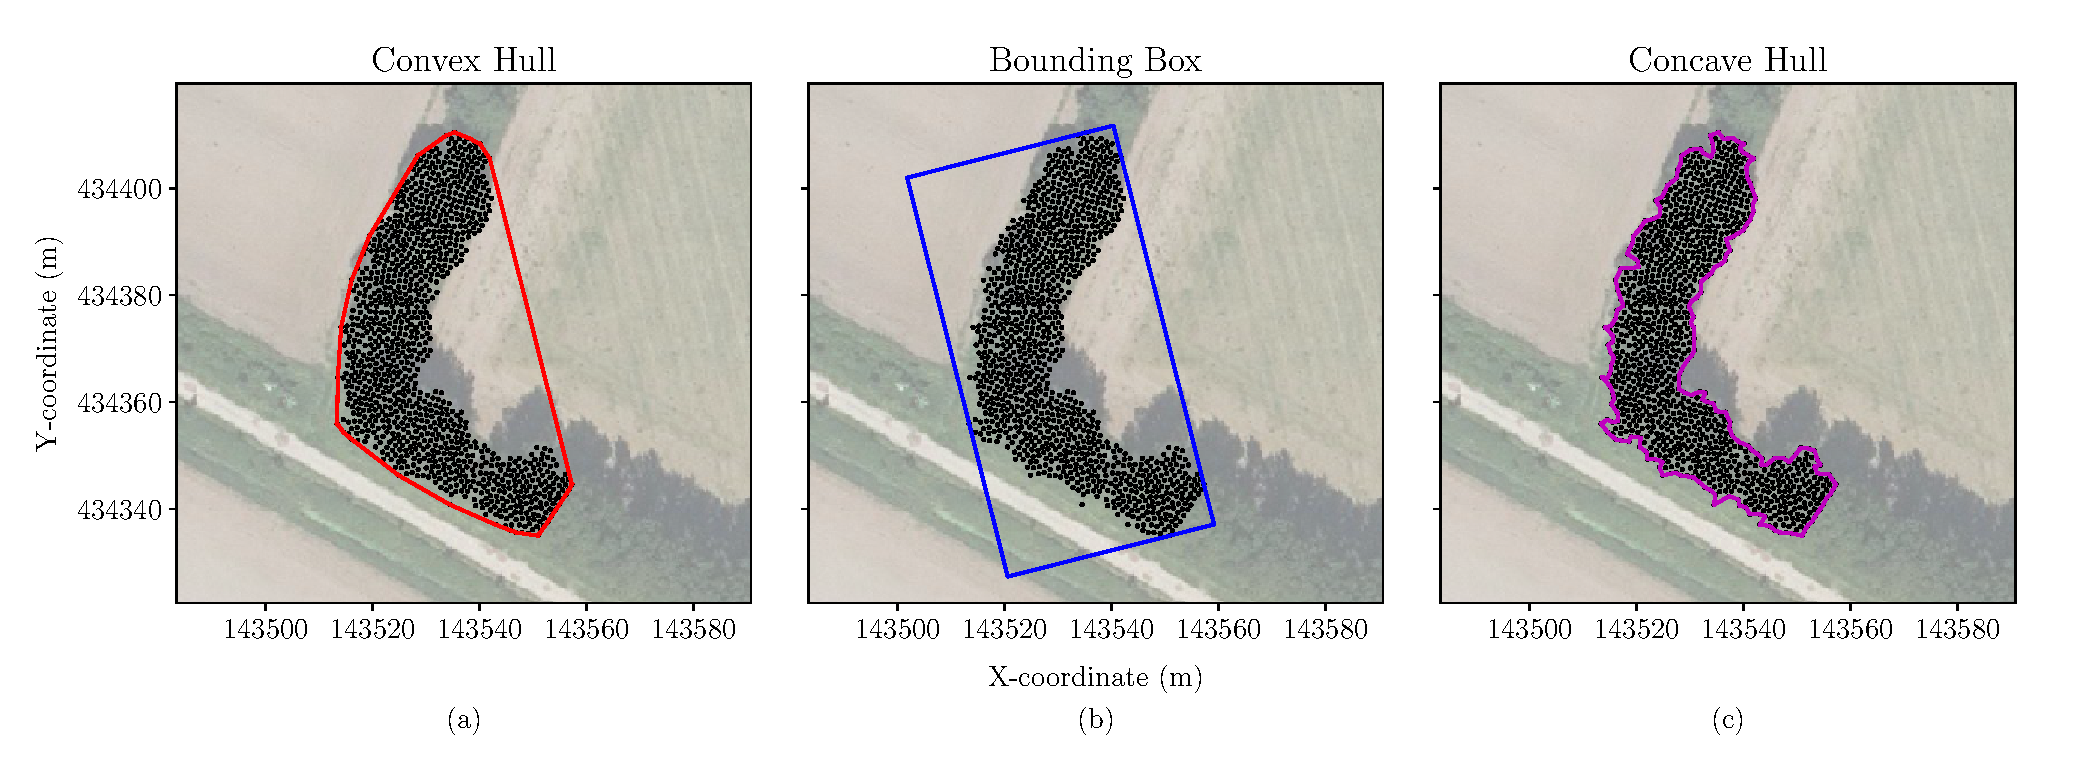
\includegraphics[scale=0.50]{./img/hulls.pdf}
%	\caption{The vegetation points of a piece of tree line within the research area are plotted on top of the high resolution orthophoto, showing the effect of downsampling the point cloud (a) and the different hulls used during the region growing algorithm: the convex hull (b), the minimal oriented bounding box (c), and the concave hull (d). During the region growing the rectangularity is calculated by dividing the area of the concave hull (d) by the area of the bounding box (c).}
%\end{figure}

\begin{figure}
	\centering
	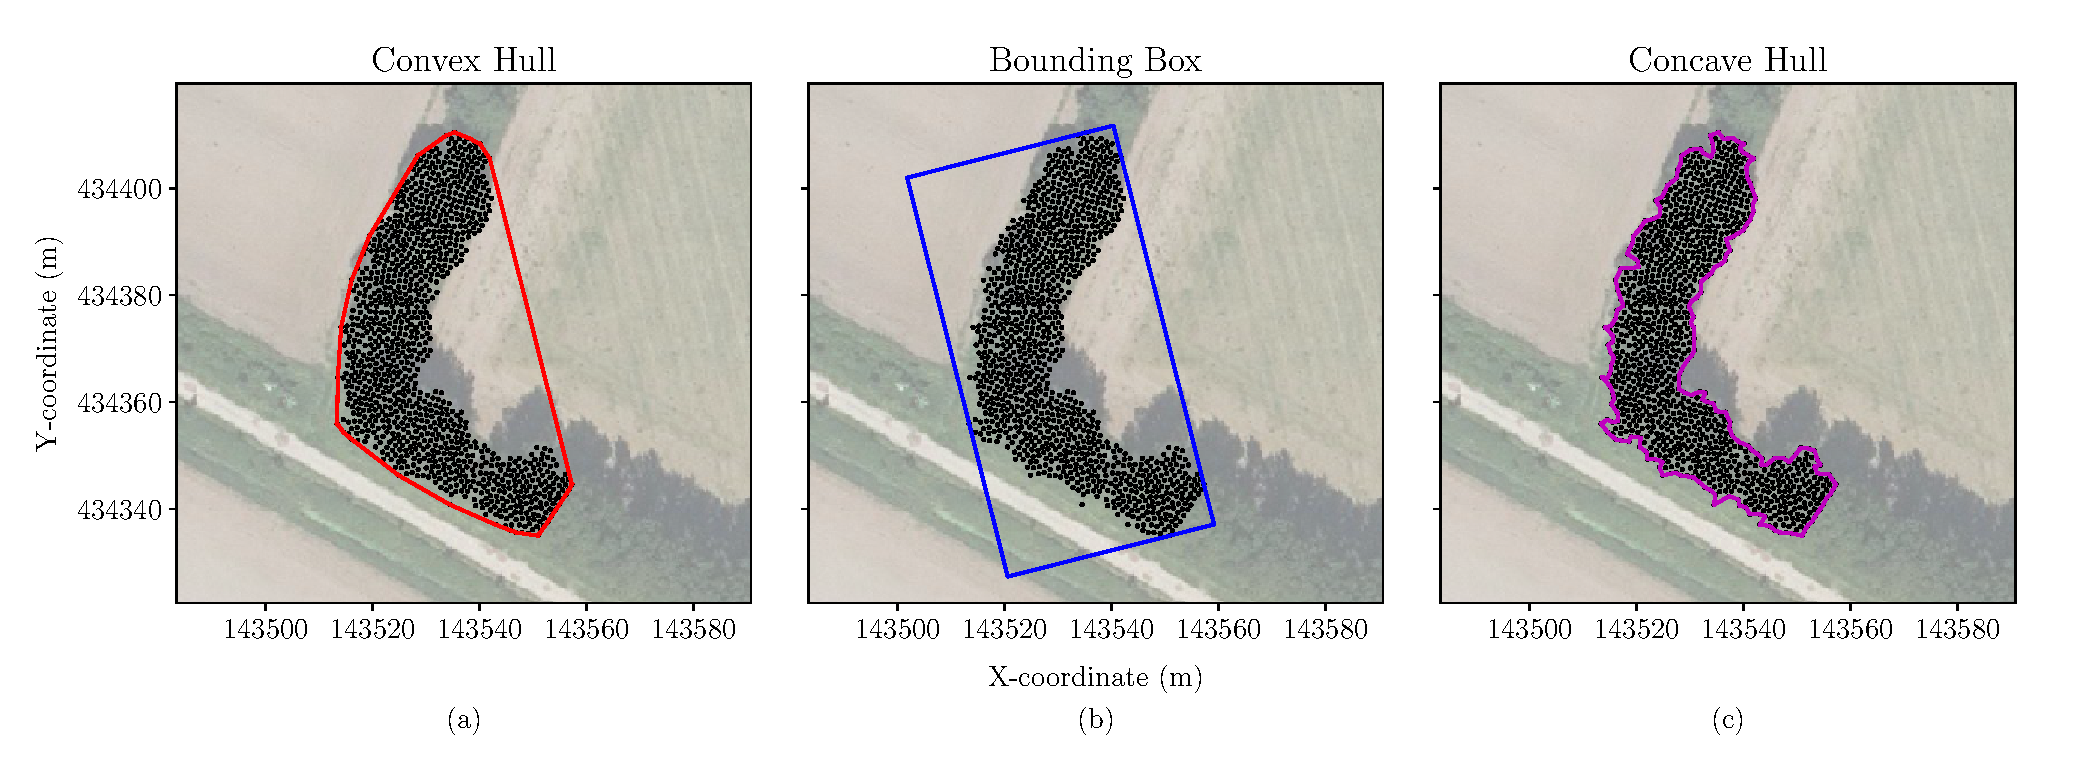
\includegraphics[width=\columnwidth]{./img/hulls.pdf}
	\caption{The downsampled vegetation points of a piece of tree line within the study area  plotted on top of the high resolution orthophoto in Rijksdriehoek-coordinates, showing the different hulls used during the region growing algorithm: (a) the convex hull, (b) the minimal oriented bounding box, and (c) the concave hull. During the region growing the rectangularity is calculated by dividing the area of the concave hull (c) by the area of the bounding box (b).}
	\label{fig:hulls}
\end{figure}

\begin{figure}
	\centering
	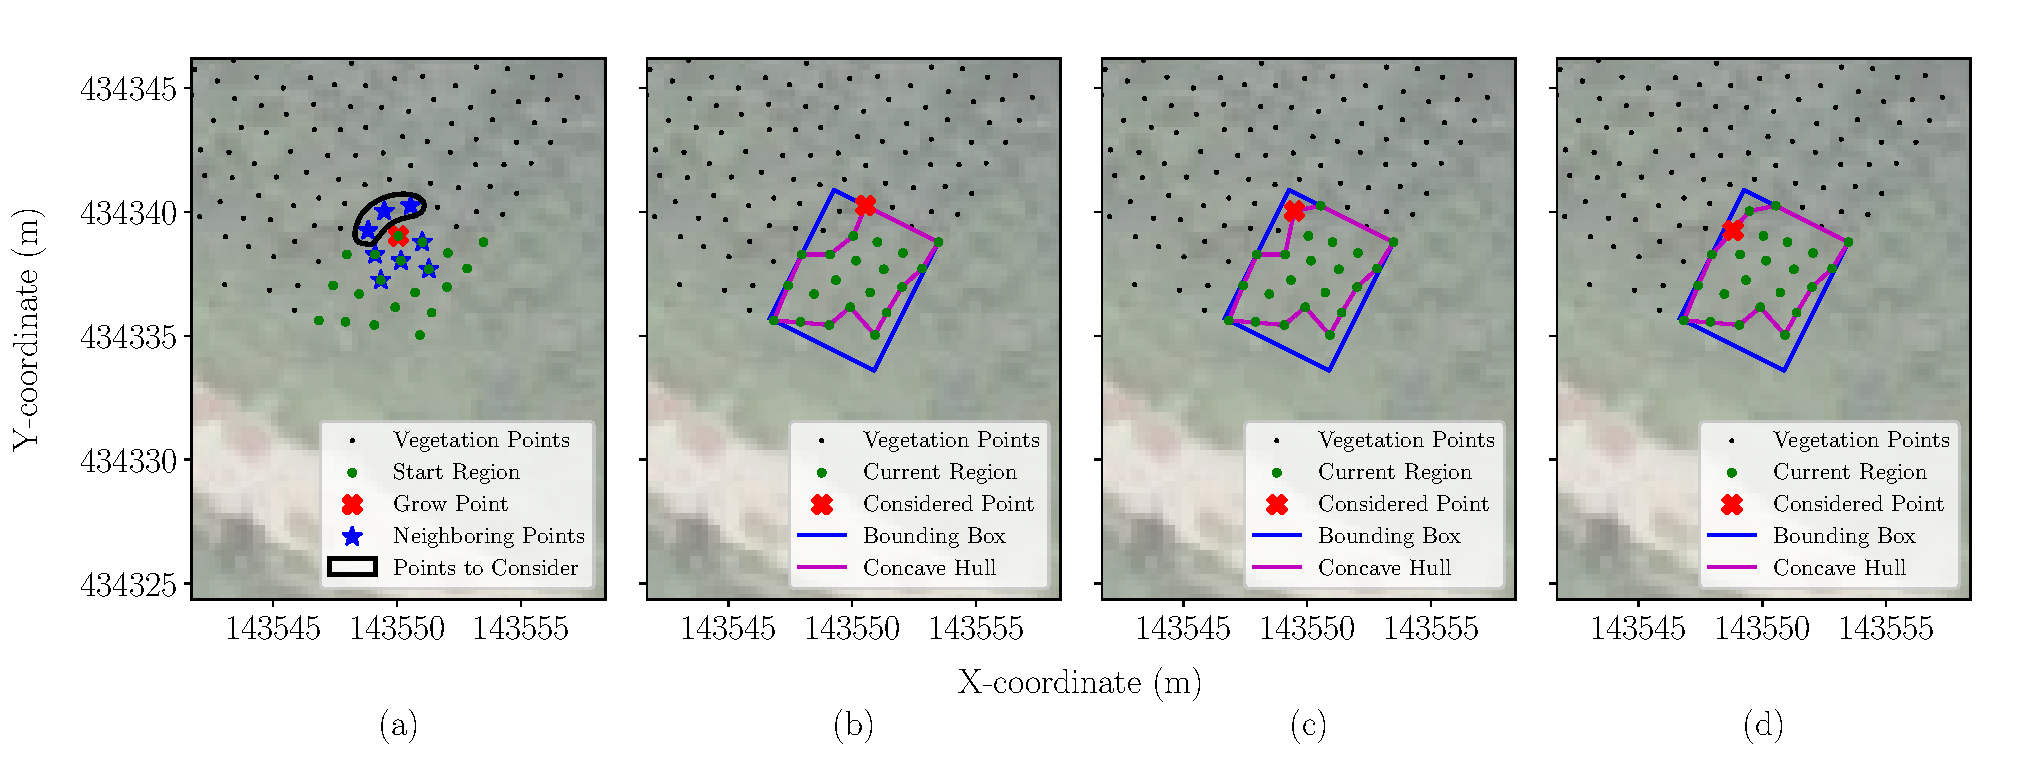
\includegraphics[width=\columnwidth]{./img/region_growing.pdf}
	\caption{An example of the region growing process for one point. First the eight nearest neighbors are computed and the neighbors which are not already part of the region are considered to be added to the region (a). A bounding box and concave hull is computed for the region with the considered point added and the rectangularity is calculated (b). If this rectangularity is above a certain threshold the point is added to the region. Subsequently the process is repeated for the other potential points (c, d). When all potential points are checked, a next point of the region is check for nearest neighbors and the whole process is repeated until all points of the region, including the ones which are added during the growing process, have been checked.}
	\label{fig:regiongrowing}
\end{figure}

\subsubsection{Object merging}
The resulting objects can be fragmented, for example, as the result of minor curves in the linear elements or small interruptions in vegetation. These objects were merged if they were in close proximity, faced a similar compass direction, and were aligned. The compass direction was determined by computing the angle between one of the long sides of the minimum bounding box and the x-axis. The alignment was checked by comparing the angle of the line between the two center points with the directions of the objects. Once merged the lengths of the objects were added and the maximum of the widths taken as the new width.

\subsubsection{Elongatedness}
The merged objects were assessed for linearity by evaluating the elongatedness of an object, which is defined as the ratio between its length and width \citep{nagao2013structural}. The definition of a linear object is not clearly defined and consequently somewhat arbitrary. After analyzing the results using different values we set the minimum elongatedness at 1.5 and a maximum width of 60 meters, because these values made for a good extraction of linear elements, while excluding large forest-like vegetation.

\subsubsection{Accuracy assessment}
The accuracy of the delineated linear objects was assessed by calculating the user's, producer's and overall accuracy, as well as the harmonic mean of the precision and recall (F1), and MCC scores \citep{congalton2008assessing}. We manually segmented the vegetation data into linear and nonlinear objects, after converting the classified vegetation points into polygons using an alpha shape. Consequently this assessment evaluates the accuracy of the segmentation given the accuracy of the vegetation points. By differencing of the automated and manually constructed data we created a map and confusion matrix detailing the accuracy.